

\section{Введение}

% Streams
\subsection{Интерфейс потоков объектов}
\begin{frame}
\frametitle{\insertsection} 
\framesubtitle{\insertsubsection}
% Фича Java 8
% Ленивость
% Функциональный стиль
\begin{itemize}
	\item Java 8 - появление анонимных функций и \textit{java.util.stream}
	\item \textit{java.util.stream} - набор классов и интерфейсов для упрощения обработки последовательностей элементов с помощью функций высших порядков
	\inputminted{java}{code/StreamsExample.java}
	\item Аналоги в других языках - LINQ в C\#, коллекции Scala
\end{itemize}
\end{frame}
\subsection{Интерфейс потоков объектов. Реализация}
\begin{frame}
\frametitle{Части цепочки вычислений} % Table of contents slide, comment this block out
\begin{itemize}
	\item \textbf{Источник объектов}. Например, массив, коллекция, функция генератор, потоки ввода/вывода и другие.
	\inputminted{java}{code/Producer.java}
	\item \textbf{Промежуточные операции}, которые преобразуют поток объектов.
	\begin{itemize}
		\item Без состояния
		\inputminted{java}{code/Stateless.java}
		\item С состоянием
		\inputminted{java}{code/Stateful.java}
	\end{itemize}
	\item \textbf{Завершающая операция}. Операция которая завершает цепочку, выполняя какое-либо действие над объектами внутри потока.
	\inputminted{java}{code/Termination.java}
\end{itemize}
\end{frame}

\begin{frame}
\frametitle{\insertsection} 
\framesubtitle{\insertsubsection}
\begin{itemize}
	
	\item Существуют расширения $java.util.stream$ - StreamEx, jOOL. Эти библиотеки совместимы со стандартной реализацией, расширяя стандартные интерфейсы.
\end{itemize}
\end{frame}


% Stream debugging
\section{Отладка потоков объектов}
\subsection{Доступные инструменты}
\begin{frame}
\frametitle{\insertsection} 
\framesubtitle{\insertsubsection}
\begin{itemize}
	\item Точки останова (с условием)
	\item Последовательное исполнение
	\item При помощи метода peek
	\item Автоматическая конвертация в код с обычными управляющими структурами и отладка этого кода
	\item Частичное исполнение и сохранение во временную коллекцию (не во всех средах разработки)
\end{itemize}
\end{frame}

\subsection{Проблемы}
\begin{frame}
\frametitle{\insertsection} 
\framesubtitle{\insertsubsection}
Недостатки отладки интерфейса потоков объекта в сравнении с обычными управляющими структурами
\begin{itemize}
	\item Отсутствие знаний о промежуточных результатах вычислений 
	\item Нетривиальная последовательность исполнения
	\item Отсутствие информации о трансформации объектов
	\item Простые стеки вызовов
	\item Отладка исключительных ситуаций % ?
\end{itemize}
\end{frame}

\subsection{Пример использования интерфейса потоков в проекте с открытым кодом}
\begin{frame}
\frametitle{\insertsection} 
\framesubtitle{\insertsubsection}
\inputminted{java}{code/Hard.java}
\end{frame}


\section{Цель}
\begin{frame}
	\frametitle{\insertsection} 
	\framesubtitle{\insertsubsection}
	\textbf{Цель}: Расширить возможности отладчика для поиска ошибок при использовании библиотек с функциями высшего порядка.
	
	\vspace{10px}
	\textbf{Задачи:}
	\begin{enumerate}
		\item Распознавание вызова Stream API возле текущей позиции отладчика.
		\item Построение промежуточных состояний между вызовами в цепочке.
		\item Нахождение переходов между состояниями.
		\item Визуализация объектов внутри состояний и переходов для них.
	\end{enumerate}
\end{frame}

\subsection{Существующие решения}
\begin{frame}
\frametitle{\insertsection} 
\framesubtitle{\insertsubsection}
Существует расширение для отладчика Visual Studio для C\# - OzCode. Одна из его функций - отладчик для LINQ
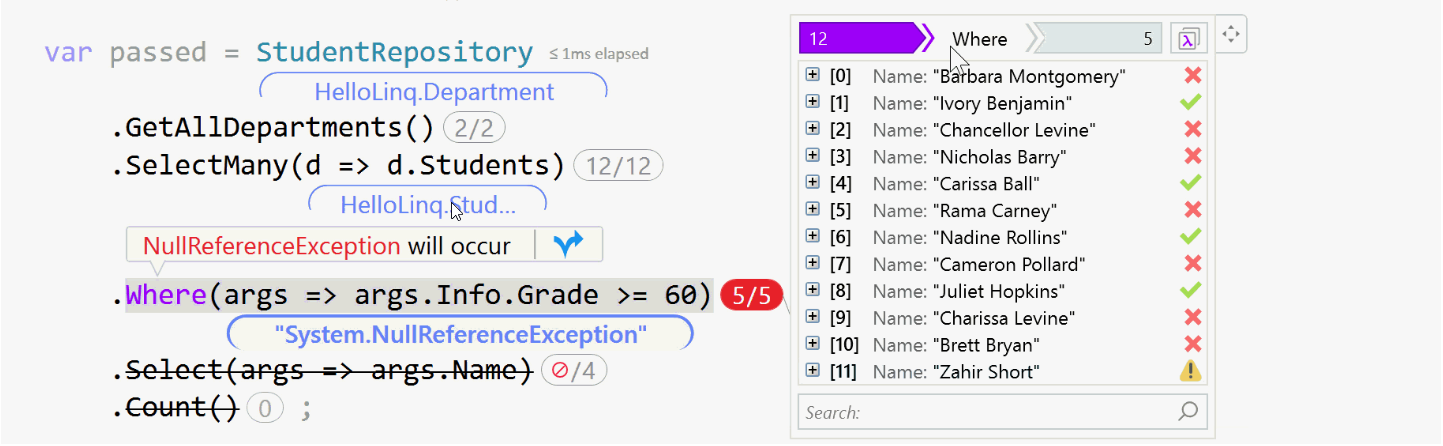
\includegraphics[scale=0.35]{img/ozcode.png}
\end{frame}

\subsection{Особенности OzCode}
\begin{frame}
\frametitle{\insertsection} 
\framesubtitle{\insertsubsection}
\begin{itemize}
	\item Работает с LINQ (язык интегрированных запросов), реализация которого отлична от реализации интерфейса потоков в Java
	\item Позволяет увидеть трансформации объектов и промежуточные результаты
	\item Закрытый исходный код
	\item Платный
	\item Только для отладчика Visual Studio
\end{itemize}
\end{frame}

\subsection{Подзадачи}
\begin{frame}
\frametitle{\insertsection} 
\framesubtitle{\insertsubsection}
\begin{enumerate}
	\item Распознать вызов Stream API возле текущей позиции отладчика.
	\item Построить промежуточные состояния между вызовами в цепочке.
	\item Построить переходы между состояниями.
	\item Визуализировать результаты.
\end{enumerate}
\end{frame}

\section{Решение}
\section{Поиск вызова}
\begin{frame}[noframenumbering]
\frametitle{\insertsection} 
\framesubtitle{\insertsubsection}
Чтобы распознать вызов будем использовать AST файла.
С учетом следующих особенностей:
\begin{itemize}
	\item Определение типа вызова: 
	\begin{itemize}
		\item Источник - первый вызов (объект), возвращающий наследника Stream<T>.
		\item Промежуточный - вызов на наследнике Stream<T>, возвращающий Stream<T>.
		\item Завершающий - вызов на наследнике Stream<T>, возвращающий что-то отличное от Stream<T>.
	\end{itemize}
	\item Цепочка может не иметь завершающей операции. Такие цепочки нам не интересны (в них нет вычислений)
	\item Может быть несколько подходящих вызовов. Необходимо найти их все.
	\item Цепочка может быть на других уровнях стека вызовов.
	\item Цепочка может быть в объемлющем коде.
\end{itemize}
\end{frame}

\subsection{Обобщение}
\begin{frame}
\frametitle{\insertsection} 
\framesubtitle{\insertsubsection}
Такой подход можно обобщить.
Для любого промежуточного вызова запомним объекты перед и после вызова.
\begin{align*}
	&.peek(x \rightarrow store(x, time)) \\
	&.call(...)\\
	&.peek(z \rightarrow \{time.increment()\})\\
	&.peek(y \rightarrow store(y, time))
\end{align*}

В результате получим два множества $Before = \{(t_i, x_i)\}, After = \{(t_i, y_i)\}$. 

Чтобы найти переходы достаточно построить \textbf{отображения}
\begin{align*}
	(t_i, x_i) \rightarrow List[(t_j, y_j)], \ \forall (t_i, x_i) \in Before \\
	(t_i, y_i) \rightarrow List[(t_j, x_j)], \ \forall (t_j, y_j) \in After
\end{align*}

\end{frame}

\subsection{Пример}
\begin{frame}
\frametitle{\insertsection} 
\framesubtitle{\insertsubsection}
Рассмотрим в качеству примера вызов:
\inputminted{java}{code/FlatMapFactorizeExample.java}
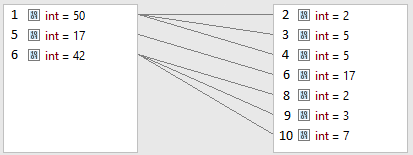
\includegraphics[scale=0.8]{img/flatMapExample.png}

Решая такие же задачи и для остальных методов, сможем получить отображения для всех. (с возможностью легко расширить набор поддерживаемых методов, например, поддержав сторонние библиотеки)
\end{frame}

\subsection{Вычисление}
\begin{frame}
\frametitle{\insertsection} 
\framesubtitle{\insertsubsection}
Выполнение кода трассировки.
\begin{enumerate}
	\item Построить выражение с дополнительными вызовами peek и обработкой собранной информации.
	\item Скомпилировать новый класс, в котором будет код, вычисляющий выражение.
	\item Загрузить его в виртуальную машину и выполнить.
	\item Получить результат вычислений и интерпретировать его.
\end{enumerate}
\end{frame}


\section{Результаты}
\begin{frame}
\frametitle{Что сделано}
TODO: простой трассирующий плагин
\end{frame}

\begin{frame}
\frametitle{\insertsection} 
\framesubtitle{\insertsubsection}
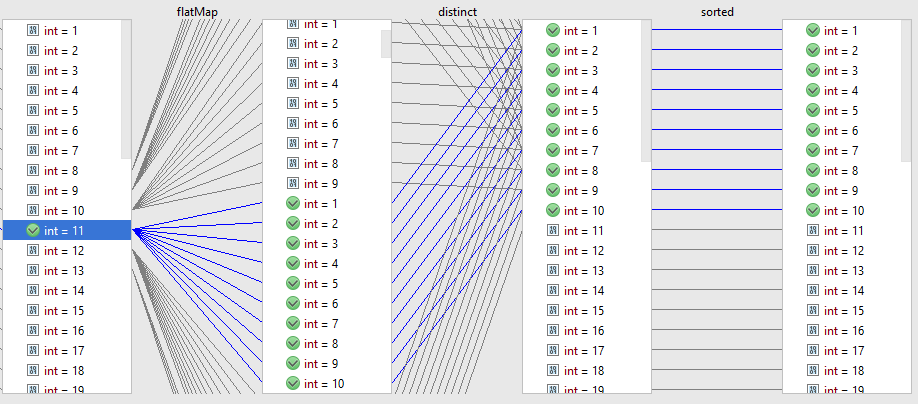
\includegraphics[scale=0.5]{img/trace-view.png}
\end{frame}


\appendix
\section{Архитектура отладчика}
\begin{frame}[noframenumbering]
\frametitle{\insertsection} 
\framesubtitle{\insertsubsection}
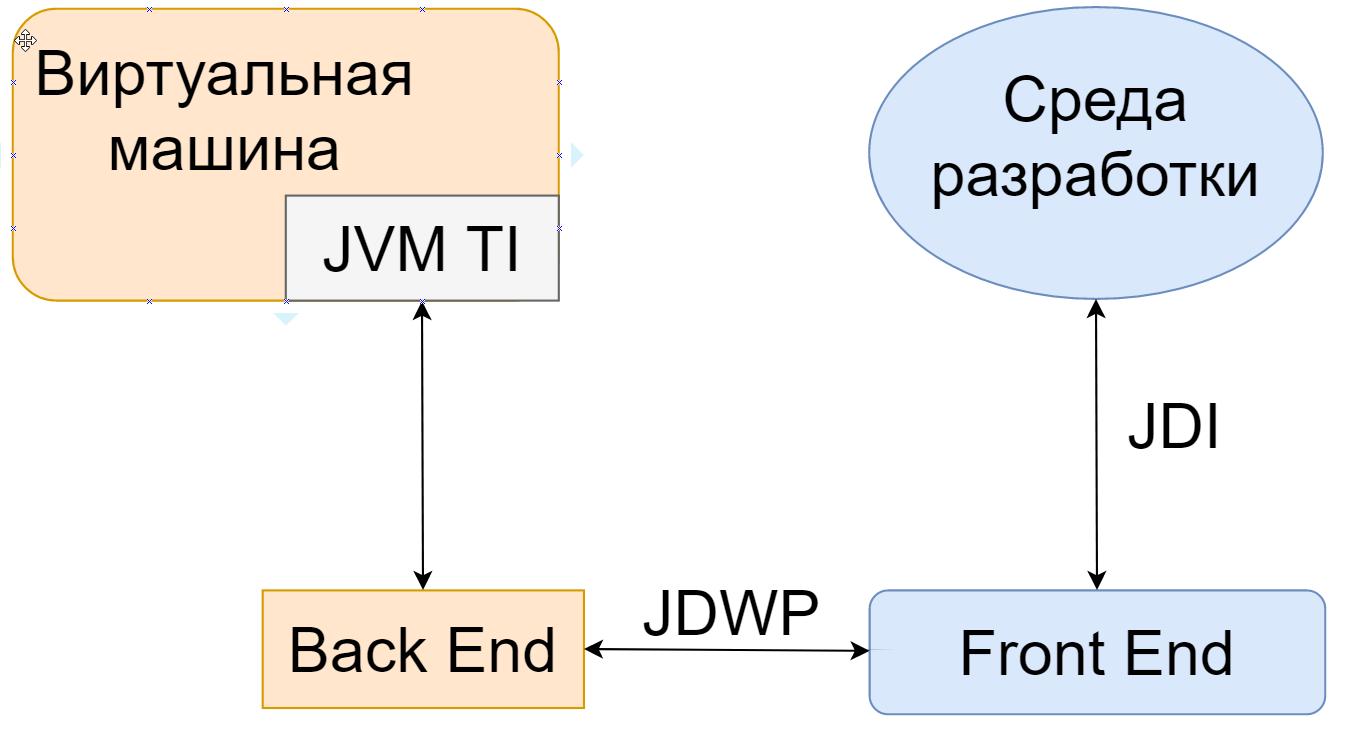
\includegraphics[scale=0.315]{img/jdpa.png}
\end{frame}
\section{Выражение для вычисления}
\begin{frame}[noframenumbering]
\frametitle{\insertsection} 
\framesubtitle{\insertsubsection}
Чтобы вычислить выражение для отслеживания исполнения цепочки потоков объектов нужно определить класс, а так же учесть следующие особенности
\begin{itemize}
	\item Поля и методы этого класса.
	
	\item Расположение класса: пакет, объемлющий класс.
	
	\item Доступ к полям и методам объемлющего класса.

	\item Доступ к приватным членам класса из лямбд и анонимных классов.

	\item Минимизация дальнейших обращений к виртуальной машине.
\end{itemize}

\inputminted{java}{code/EvalClass.java}
\end{frame}

\section{Гарантии библиотеки}
\begin{frame}
\frametitle{\insertsection} 
\framesubtitle{\insertsubsection}
\begin{itemize}
	\item Поток объектов ленивый. Это значит, что объекты не из источника будут браться только когда выполняется терминальная операция и ей нужен объект.
	\item Это исключает ситуации, когда из каких-то промежуточных операций требовались объекты, но затем не использовались
	\item Но это не исключает, что некоторым промежуточным операциям потребуется прочитать более одного объекта, чтобы вернуть один. (см sorted, distinct, и др)
	\item Следствие: нет вызова терминальной операции - нет вычислений
\end{itemize}

\end{frame}
\section{Требования к коду пользователя}
\begin{frame}[noframenumbering]
\frametitle{\insertsection} 
\framesubtitle{\insertsubsection}
\begin{itemize}
	\item "Streams are lazy; computation on the source data is only performed when the terminal operation is initiated, and source elements are consumed only as needed."
	\item Это значит, что объекты не могут браться из источника только по необходимости. % ситуация, когда из каких то промежуточных операций забрались объекты, но затем не использовались исключены
	\item Но это не исключает, что некоторым промежуточным операциям потребуется прочитать всё объекты. (см sorted, distinct, и др)
\end{itemize}

\end{frame}
\section{Распознавание вызова}
\begin{frame}[noframenumbering]
\frametitle{\insertsection} 
\framesubtitle{\insertsubsection}
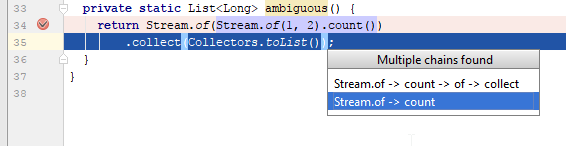
\includegraphics[scale=0.7]{img/ambiguous.png}
\end{frame}


\section{Пример}
\begin{frame}
\frametitle{\insertsection} 
\framesubtitle{\insertsubsection}
Рассмотрим пример. И поставим задачу восстановить промежуточные состояния и переходы
\inputminted{java}{code/StreamWithoutPeeks.java}
\end{frame}

\begin{frame}
\frametitle{\insertsection} 
\framesubtitle{\insertsubsection}
Интерфейс Stream для отладочных целей определяет метод peek.
\inputminted{java}{code/StreamWithPeeks.java}
\end{frame}

\begin{frame}[noframenumbering]
\frametitle{\insertsection} 
\framesubtitle{\insertsubsection}
\fboxsep=0pt
\noindent
	\begin{minipage}[t]{0.48\linewidth}
		Информация, которую можно извлечь:
		\begin{itemize}
			\item Последовательность прохождения объектов через цепочку вызовов
			\item Результат фильтрации
			\item sorted имеет состояние и требует выполнить весь поток до своего вызова
			\item Преобразования объектов
		\end{itemize}
	\end{minipage}
	\hfill%
		\begin{minipage}[t]{0.48\linewidth}
			Результат вызова:
			\inputminted{text}{code/peekResults.txt}
		\end{minipage}
\end{frame}
